\documentclass[11pt,psfig]{article}
\usepackage{epsfig}
\usepackage{times}
\usepackage{amssymb}
\usepackage{float}

\newcount\refno\refno=1
\def\ref{\the\refno \global\advance\refno by 1}
\def\ux{\underline{x}}
\def\uw{\underline{w}}
\def\bw{\underline{w}}
\def\ut{\underline{\theta}}
\def\umu{\underline{\mu}} 
\def\bmu{\underline{\mu}} 
\def\be{p_e^*}
\newcount\eqnumber\eqnumber=1
\def\eq{\the \eqnumber \global\advance\eqnumber by 1}
\def\eqs{\eq}
\def\eqn{\eqno(\eq)}

 \pagestyle{empty}
\def\baselinestretch{1.1}
\topmargin1in \headsep0.3in
\topmargin0in \oddsidemargin0in \textwidth6.5in \textheight8.5in
\begin{document}
\setlength{\parskip}{1.2ex plus0.3ex minus 0.3ex}


\thispagestyle{empty} \pagestyle{myheadings} \markright{G}



\title{CS 266 Homework 5}
\author{Zachary DeStefano, PhD Student, 15247592}
\date{Due Date: May 15}

\maketitle

\vfill\eject

\section*{Problem 10.1}

\subsection*{Part A}

Here is the algorithm:\\
Traverse binary search tree for y-coordinate until you hit a split vertex\\
Traverse right subtree:\\
- Every time you make a right turn, call the left node n and do Recurse(n)\\
Traverse left subtree:\\
- Every time you make a left turn, call the right node n and do Recurse(n)\\
\\
Recurse(n):\\
- Report intervals in the binary search tree for n that lie in our point.\\

\subsection*{Part B}

We have a binary search tree for the y-coordinate of the points, thus we will get all the segments whose y-coordinates are in the y-coordinate range of our vertical segment and only those segments where the y-coordinates match. Once we establish the y-range, we have interval trees for all the x-coordinates of the segments. Querying the interval tree will ensure we get all the segments where the x-coordinate matches and only those segments. Since the segments will match both the x and y coordinates and only those matching segments are retrieved, the query will be correct. 

\newpage

\subsection*{Part C}

Preprocessing: \\
The binary search tree can be constructed in $O(n \cdot log(n))$\\
Each segment tree can be constructed in $O(m \cdot log(m))$ time where $m$ is the number of intervals. \\
At each level $k$ of the binary search tree, there are at most $2^k$ nodes and each node has $\frac{n}{2^k}$ intervals, thus the run time per level is $2^k(\frac{n}{2^k} log(\frac{n}{2^k}))$\\
Thus each level takes $O(n \cdot log(n))$ time to compute and there are $log(n)$ levels. \\
The running time is thus $n \cdot log(n) + n \cdot log^2(n)$\\
In summary, it take $O(n \cdot log^2(n))$ time for preprocessing  \\
\\
Query: \\
It may traverse up to $log(n)$ nodes in the range tree. \\
For each node, traversing the associated interval tree will take $O(log(n))$ time. \\
We thus have a query time of $O(log^2(n))$\\
\\
Storage:\\
A binary search tree on the y-coordinate can be stored in $O(n)$ space. \\
An interval tree can be stored in $O(m)$ space where $m$ is number of intervals. \\
At each level $k$ of the binary search tree, there are at most $2^k$ nodes and each node has $\frac{n}{2^k}$ intervals, thus the storage per level is $2^k(\frac{n}{2^k})=n$\\
Thus each level uses $O(n)$ storage and there are $log(n)$ levels. \\
The total storage is thus $n + n \cdot log(n)$\\
In summary, $O(n \cdot log(n))$ storage is required

\newpage

\section*{Problem 10.6c}
Construct a binary search tree of the endpoints. \\
For each leaf in the Binary Search Tree, store the number of overlapping intervals. \\
\\
Construction algorithm:
\begin{verbatim}
-Make a Binary Search Tree of Endpoints
-Sort the list of endpoints
-Initialize currentCount to zero
-For each endpoint in ascending order:
-     If left endpoint:
-          Add one to currentCount
-     If right endpoint:
-          Subtract one from currentCount
-     Put currentCount into endpoint node in Binary Search Tree
\end{verbatim}
Query algorithm to get number of intervals at point q:\\
1. Traverse binary search tree until you find the greatest endpoint that is less than q\\
2. Report its count. \\
\\
Analysis:\\
Construction will be $O(n \cdot logn)$ \\
Query will be $O(logn)$ since it is still a binary search tree \\
Storage will be $O(n)$ since it is just a binary search tree with an added data field in the nodes
\newpage
\section*{Problem 14.6}

There is no way to do a triangulation that will fit that criteria. In the worst case, we will have a square and it will be next to a square that is one fourth its size and the vertices need to be triangulated. We will thus have a point P that is one fourth the way along one of the sides of the triangle. \\
\\
If P is connected to the center point, then an obtuse angle ends up being formed with the side. Here is an illustration of how it happens:
\begin{figure}[H]
\centering
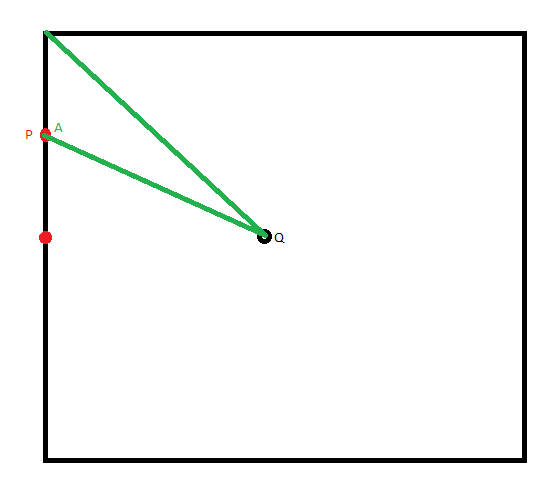
\includegraphics[height=4in]{hw5prob3_diagram1.png}
\caption{Proposed Triangulation. Angle A will be obtuse, violating requirements}
\end{figure}
If we have an interior point that is not the center, then its triangulation has an obtuse angle, violating the constraints. This is because it has to be connected to the 4 corner points, meaning there are 4 triangles whose angle sum needs to add to 360. Since they are not all 90 degrees if it is not the center point, at least one of them must be greater than that.
\begin{figure}[H]
\centering
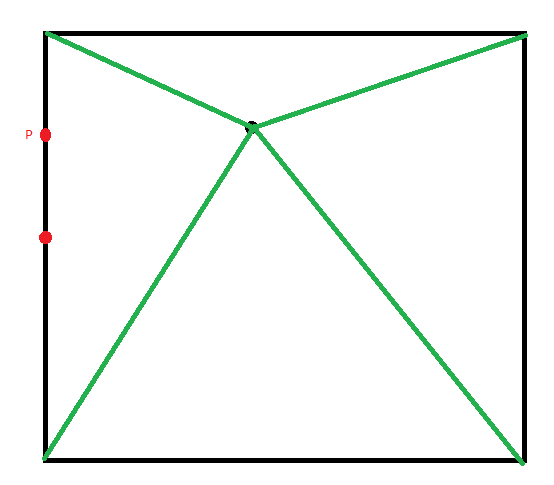
\includegraphics[height=4in]{hw5prob3_diagram2.png}
\caption{Proposed Triangulation. At least one interior angle will be obtuse}
\end{figure} 
Finally, we cannot connect P to any of the vertices on its own side since it is already connected there. Therefore, the last remaining vertices it might be possible to connect it to are the vertices on the opposite side. Lets call them $R$ and $S$ where $R$ is the one that lies closer to $P$. If we connect $P$ to $S$ or $P$ to $R$ then in both cases we end up with right triangles that violate our constraints. 
\begin{figure}[H]
\centering
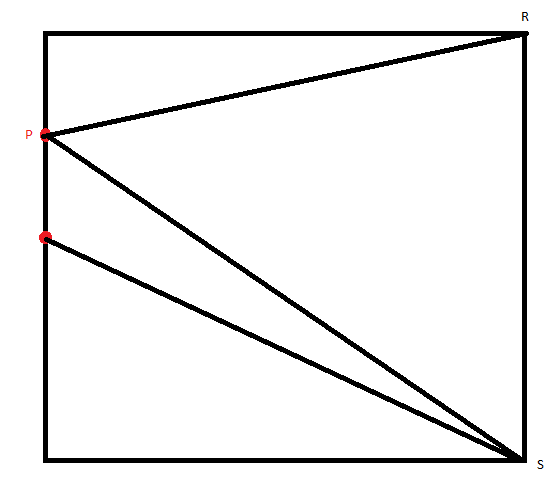
\includegraphics[height=4in]{hw5prob3_diagram3.png}
\caption{Proposed Triangulation. The triangles formed will violate the constraints}
\end{figure} 
There is one last case we need to consider. We have established that we need the interior center point. We have not proven that adding an extra interior point is not possible. Consider the triangulation that results after getting the interior center point:
\begin{figure}[H]
\centering
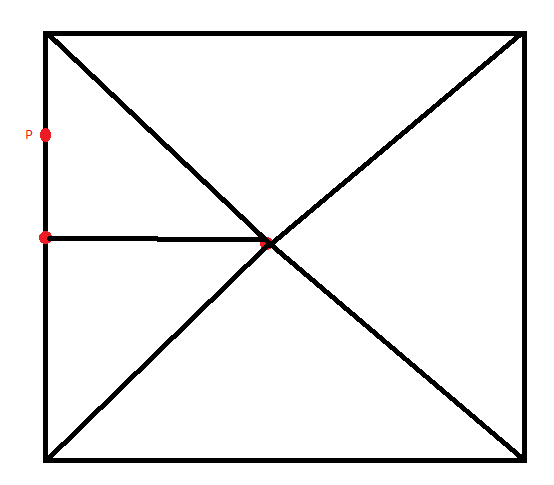
\includegraphics[height=4in]{hw5prob3_diagram4.png}
\caption{Proposed Triangulation}
\end{figure}  
We cannot add any points on the existing boundaries because then our triangles will become quadrilaterals. We will end up not being able to triangulate those quadrilaterals for the same reason that we cannot triangulate the quadrilateral we currently have, which is explained in the next paragraph.\\
\\
Let's say we try to add interior points $Q$ and $R$. When we add $Q$, we will have to connect it to the 4 points on the boundary. The total of the angles around $Q$ must be 360 and there are only 4 angles. Since we are not inside a square, they cannot all be 90 degrees, so at least one of them will be greater than 90 degrees. If we try to add a point $R$ to split up that angle, we are inside a triangle, so there are only 3 points to connect $R$ to, meaning that there are only 3 angles around $R$ that add to 360, thus one of them will violate the constraint. We are faced with the same problem if we try to add more interior points. This proves that adding interior points will not be a solution. 
\begin{figure}[H]
\centering
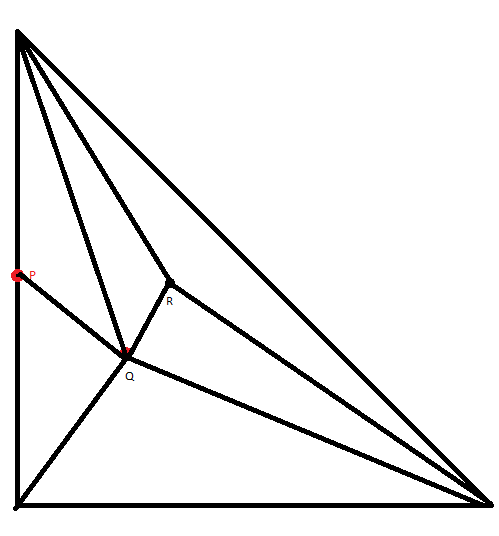
\includegraphics[height=4in]{hw5prob3_diagram5.png}
\caption{There is no way to add Q and R here without violating constraints}
\end{figure}  
Since we have run out of places to connect P to, it is not possible to do the triangulation as specified.
\newpage

\section*{Problem 14.12}

For this algorithm, a vertex v in the quad tree will have this data:\\
- $subtree(i)$ for i=1,2,3,4 will be pointers to subvertices if this square is split up\\
- $value$ will be intensity value if this vertex is a leaf. \\
$J_1$, $J_2$ will denote the quad trees for the images and will point to the root vertex \\
\\
The idea behind this algorithm is that we can traverse the two quad trees concurrently to compute the AND and OR quad trees and potentially take shortcuts. If we are computing the AND tree and we encounter a 0, then we already know that the entire square in the result image will be 0. Similarly, if we are computing the OR tree and we encounter a 1, then we already know that the entire square in the result image will be 1. If we are computing the AND tree and encounter a 1, then the result will be entirely dependent on the other tree. Similarly, if we are computing the OR tree and encounter a zero, then the result is entirely dependent on the other tree.\\
\\
Here are the algorithms in detail:\\
Run GetANDQuadTree($J_1$,$J_2$) and GetORQuadTree($J_1$,$J_2$)
\begin{verbatim}
GetANDQuadTree(I,J):
-     Initialize vertex v with no subtrees or values
-     if both I,J have subtrees:
-          for each subtree i from 1 to 4:
-               v.subtree(i) = GetANDQuadTree(I.subtree(i),J.subtree(i))
-          return v
-     else if both I,J are leaves:
-          v.value = (I.value and J.value)
-     else:
-          let K_1 be the one that is a leaf
-          let K_2 be the one that has a subtree
-          if K_1.value is 0:
-               v.value = 0
-               return v
-          else:
-               for each subtree i from 1 to 4:
-                    v.subtree(i)=K_2.subtree(i)
-               return v
\end{verbatim}
\newpage
\begin{verbatim}
GetORQuadTree(I,J):
-     Initialize vertex v with no subtrees or values
-     if both I,J have subtrees:
-          for each subtree i from 1 to 4:
-               v.subtree(i) = GetORQuadTree(I.subtree(i),J.subtree(i))
-          return v
-     else if both I,J are leaves:
-          v.value = I.value or J.value
-     else:
-          let K_1 be the one that is a leaf
-          let K_2 be the one that has a subtree
-          if K_1.value is 1:
-               v.value = 1
-               return v
-          else:
-               for each subtree i from 1 to 4
-                    v.subtree(i)=K_2.subtree(i)
-               return v

\end{verbatim}


%\begin{figure}[H]
%\centering
%\includegraphics[height=4in]{prob1plot.jpg}
%\caption{Probability of Class Labels with decision boundaries marked}
%\end{figure}


\end{document}








